\section{Zadanie 5}
\subsection{Opis problemu}
Zadanie polegało na wygenerowaniu wykresów wielomianów interpolowanych z poniższych funkcji za pomocą wcześniej zaimplementowanych metod.
\begin{enumerate}
  \item $f(x) = e^x, [0, 1], n = 5, 10, 15$
  \item $g(x) = x^2 \sin(x), [-1, 1], n = 5, 10, 15$
\end{enumerate} 
\subsection{Rozwiązanie}
Na poniższych rysunkach przedstawiłem wykresy dla funkcji $f(x)$ oraz $g(x)$ dla poszczególych $n = 5, 10, 15$ 
\begin{figure*}
  \begin{multicols}{2}
        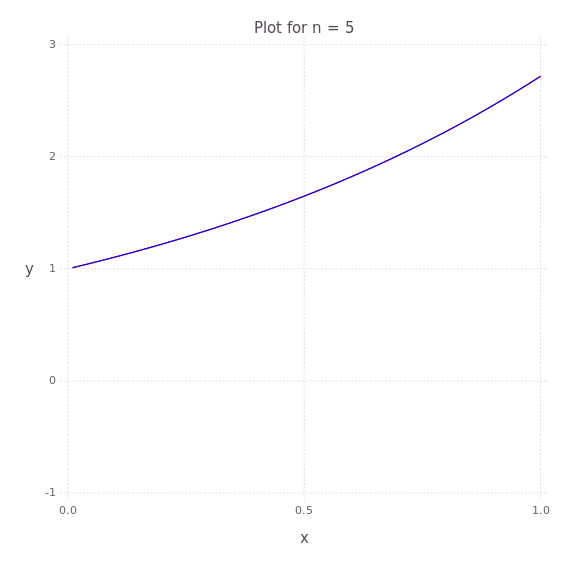
\includegraphics[width=\linewidth]{../task-5/plots/myplot-ex-5.png}\par 
        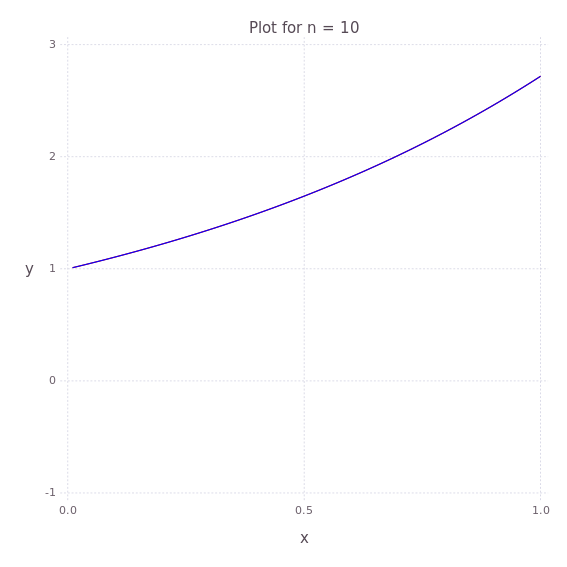
\includegraphics[width=\linewidth]{../task-5/plots/myplot-ex-10.png}\par 
    \end{multicols}
    \begin{multicols}{2}
        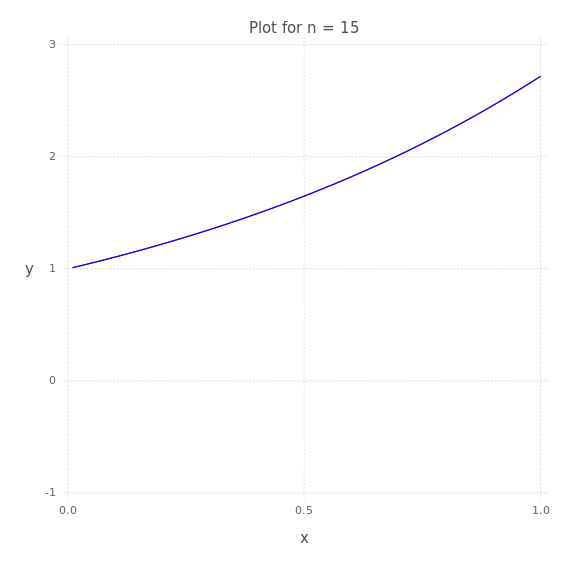
\includegraphics[width=\linewidth]{../task-5/plots/myplot-ex-15.png}\par 
    \end{multicols}
    \caption{Wykresy dla $f(x) = e^x$}    
\end{figure*}
\begin{figure*}
    \begin{multicols}{2}
        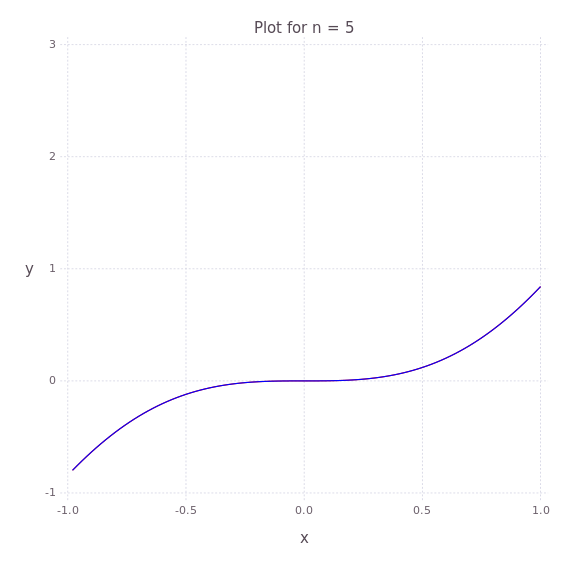
\includegraphics[width=\linewidth]{../task-5/plots/myplot-x2sinx-5.png}\par 
        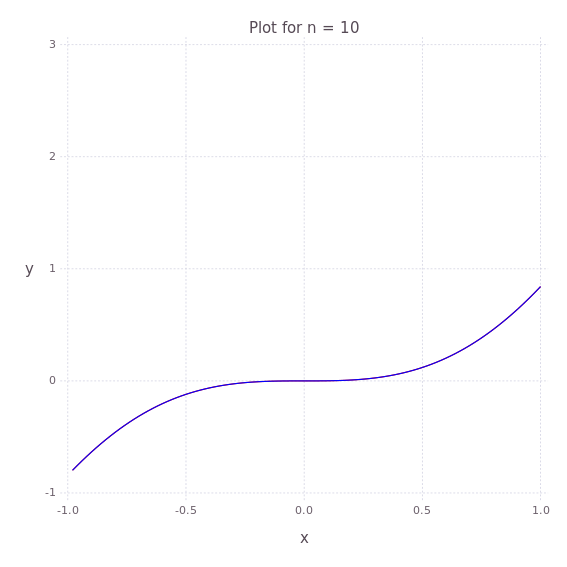
\includegraphics[width=\linewidth]{../task-5/plots/myplot-x2sinx-10.png}\par           
    \end{multicols}
    \begin{multicols}{2}
        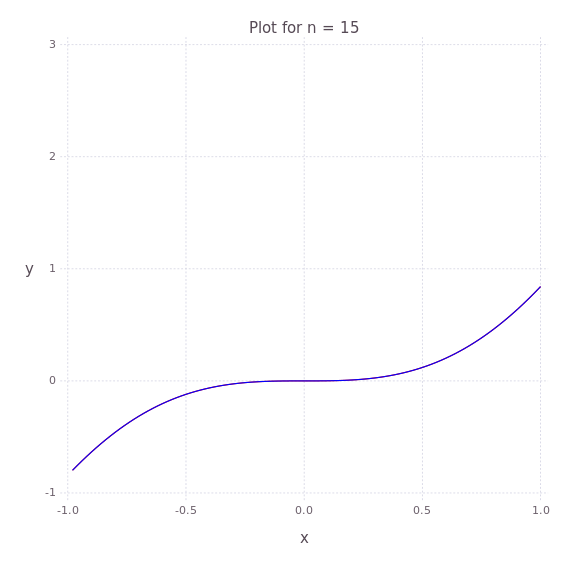
\includegraphics[width=\linewidth]{../task-5/plots/myplot-x2sinx-15.png}\par
    \end{multicols}
    \caption{Wykresy dla $g(x) = x^2 \sin(x)$}    
\end{figure*}
\subsection{Analiza wyników}
W przypadku przykładów z zadania piątego, wykresy wielomianów będących interpolacją funkcji pokryły się z wykresami tych funkcji. Interpolacja poprawnie - z pewnym małym błędem - odwzorwała zadane funkcje. Funkcje interpolowane nie spełniały żadnych warunków, które mogły powodować efekt Rungego\footnote{Efekt opisany w analizie kolejnego zadania}, mimo tego, że odległość między poszczególnymi węzłami jest stała i ich ilość nie gęstniała na krańcach przedziału.